% METHODS

\noindent The layered LED sample is shown in \autoref{fig:metal_layers} was grown by the staff of the course.
To form working LEDs from the wafer, the following steps were done at NTNU NanoLab:

\begin{enumerate}
    \item Front contact formation
    \item GaAs contact layer etch
    \item Backside contact formation
    \item Mesa etch, PECVD passivation deposition, and contact annealing
    \item Planarization and passivation layer etch
    \item Pad metallization
\end{enumerate}

\begin{figure}[ht]
    \centering
    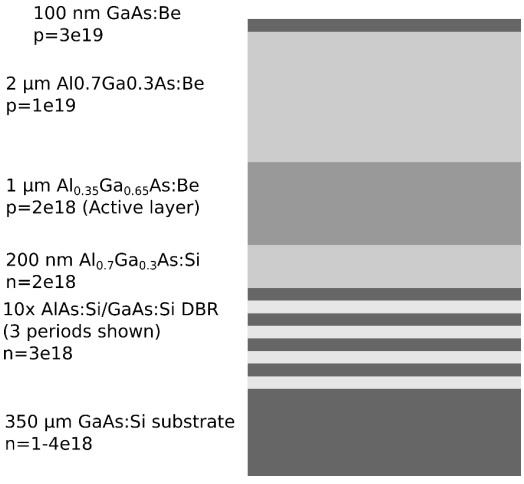
\includegraphics[width=0.45\textwidth]{figures/metal_layers.jpg}
    \caption{
        The layered LED sample made by the staff of the course.
        The layers were grown in the MBE, molecular beam epitaxy, machine at NTNU NanoLab.
        Figure borrowed from the lab manual \cite{labmanual}.
    }
    \label{fig:metal_layers}

\end{figure}

Each step was first done with a GaAs dummy sample to check that the process was working as intended.
After the last step, the IV-characteristics of the LEDs were inspected.
%After the last step, the LED was tested at a lab at IES, the Department of Electronic Systems at NTNU.


\subsection{LED design}
\label{methods:led_design}

Different finger spacings and finger widths were tested.
An overview schematic of the LED design is shown in \autoref{fig:led_schematic}.
One LED was 1 mm x 1 mm.
The bus bar for contact pad was 1 mm x 40 \textmu m.
The bus bar connecting the fingers was 1 mm x 30 \textmu m.
The fingers were 500 \textmu m long, with widths at 4, 8, 12 and 16 \textmu m, and finger spacings at 40, 60, 80 and 100 \textmu m.
The first lithography layer is shown in \autoref{fig:CleWin_L1}.
The second lithography layer, \autoref{fig:CleWin_L2}, was equal to the first, but scaled with a 5 \textmu m buffer everywhere to protect the fingers. 
The third lithography layer, \autoref{fig:CleWin_L3}, was for the mesa etch, and was a box around each LED with a 6 \textmu m buffer. 
The fourth lithography layer, \autoref{fig:CleWin_L4}, was for the etch of the passivation layer, and was a 30 \textmu m x 980 \textmu m box on each bottom bus bar. 
The fifth and final lithography layer, \autoref{fig:CleWin_L5}, was for the pad metallization, and was a 1000 \textmu m x 800 \textmu m box at the bottom of each LED connected to the bottom bus bar.
Schematics of the different layers are shown in \autoref{fig:CleWin_L1} to \autoref{fig:CleWin_L5}.
Schematics of the alignment marks in layer 1 and layer 2 is shown in \autoref{fig:CleWin_alignment_marks}.

\begin{figure}[ht]
    \centering
    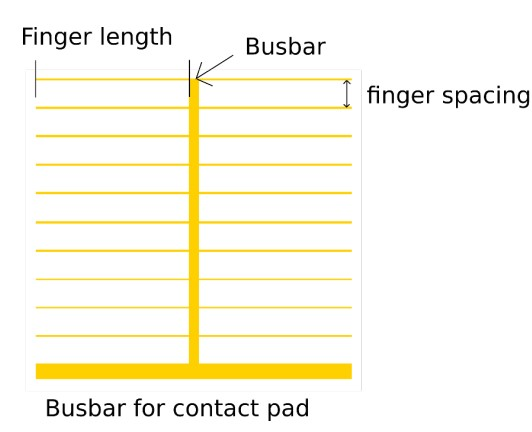
\includegraphics[width=0.45\textwidth]{figures/LED_schematic.jpg}
    \caption{
        Schematic of the LED design.
        Figure borrowed from the lab manual.
    }
    \label{fig:led_schematic}
\end{figure}

% clewin figures, L1 to L5 and alignment marks




\subsection{Front contact formation}
\label{methods:front_contact}

The bus bars and their fingers, i.e. the front contacts, were formed with lithography and lift-off.
A dose test was done to find the optimal dose and developing time for the resist, ensuring an undercut.
To verify this, both a SEM image and optical images of the sample were taken.
The optimal dose for MAN 440 was 1300 mJ/cm$^2$ and the optimal developing time was 5 minutes.
The hot plate temperatures are from the NanoLab hot plates in the student lab area, which have not been calibrated in a long time and can have some uncertainties. 
Negative photoresist was used, and the steps were done in the following order:
\begin{enumerate}
    \item Cleaned the sample with acetone and IPA.
    \item Dehydration baked at 150 \textdegree C for 5 minutes.
    \item Spin coated MAN 440 resist at 4000 rpm for 30 seconds with 1000 rpm/s acceleration.
    \item Cleaned the backside.
    \item Soft baked at 95 \textdegree C for 1 minute.
    \item Exposed the pattern at 1300 mJ/cm$^2$ in the MLA.
    \item Developed in maD-332S developer for 5 minutes.
    \item Optical inspected the pattern.
    \item Teaching assistants metallized the wafer with a \\Pd/Ti/Pt/Au stack.
    \item Lift-off with acetone.
\end{enumerate}

The Pd/Ti/Pt/Au stack is referred to as the Au fingers. 

Unfortunately, a mix-up of the type of developer was done, and the process had to be repeated. 
The optical inspection before round number two showed some contamination on the wafer, which was probably caused by the wrong developer.
The wafer was cleaned thoroughly with acetone and IPA before the second round, but some contamination might have been left behind.

Another problem was that the dose test were done with a resist that got emptied, and a newer resist had to be used for the actual process.
When using the new resist the developer time was increased from 5 to 6 minutes, which gave an undercut but damaged the alignment marks and the thickest and closest fingers.

\begin{figure}[h]
    \centering
    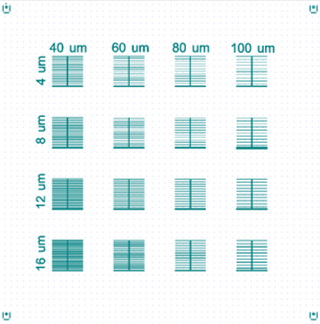
\includegraphics[width=0.3\textwidth]{figures/CleWin_L1.png}
    \caption{
        Layer 1. 
        Numbers on the top is the spacing between the fingers in the LED matrix.
        Numbers on the left side is the width of the fingers in the LED matrix.
        Each LED is 1 mm x 1 mm. 
        Alignment marks for layer 1 are in the corners. 
    }
    \label{fig:CleWin_L1}
\end{figure}


% L2
\begin{figure}[h]
    \centering
    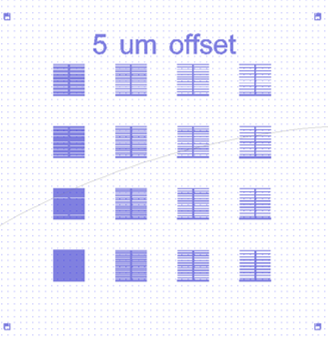
\includegraphics[width=0.3\textwidth]{figures/CleWin_L2.png}
    \caption{
        Layer 2. 
        This is the same as layer 1, but with a 5 \textmu m buffer on the whole pattern. 
    }
    \label{fig:CleWin_L2}
\end{figure}


% L3 
\begin{figure}[h]
    \centering
    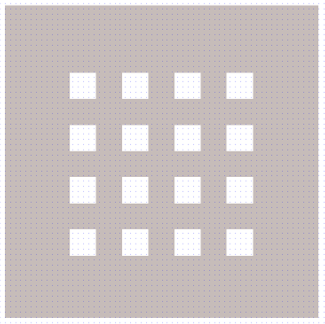
\includegraphics[width=0.3\textwidth]{figures/CleWin_L3.png}
    \caption{
        Layer 3. 
        This is the mesa etch layer. 
        The size of the box covering each LED is 1.012 mm x 1.012 mm.
    }
    \label{fig:CleWin_L3}
\end{figure}

% L4
\begin{figure}[h]
    \centering
    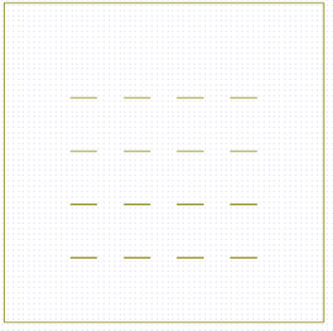
\includegraphics[width=0.3\textwidth]{figures/CleWin_L4.png}
    \caption{
        Layer 4. 
        This is the HF etch layer. 
        Each bar is covering a part of the bottom bus bar, with a size of 30 \textmu m x 980 \textmu m.
    }
    \label{fig:CleWin_L4}
\end{figure}

% L5
\begin{figure}[]
    \centering
    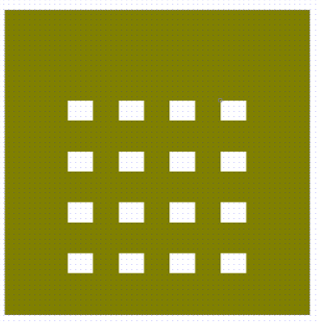
\includegraphics[width=0.3\textwidth]{figures/CleWin_L5.png}
    \caption{
        Layer 5. 
        This is the pad metallization layer, where each box is 1 mm x 0.8 mm. 
        The box is covering the bottom bus bar of each LED. 
    }
    \label{fig:CleWin_L5}
\end{figure}


% Alignment marks
\begin{figure}[]
    \centering
    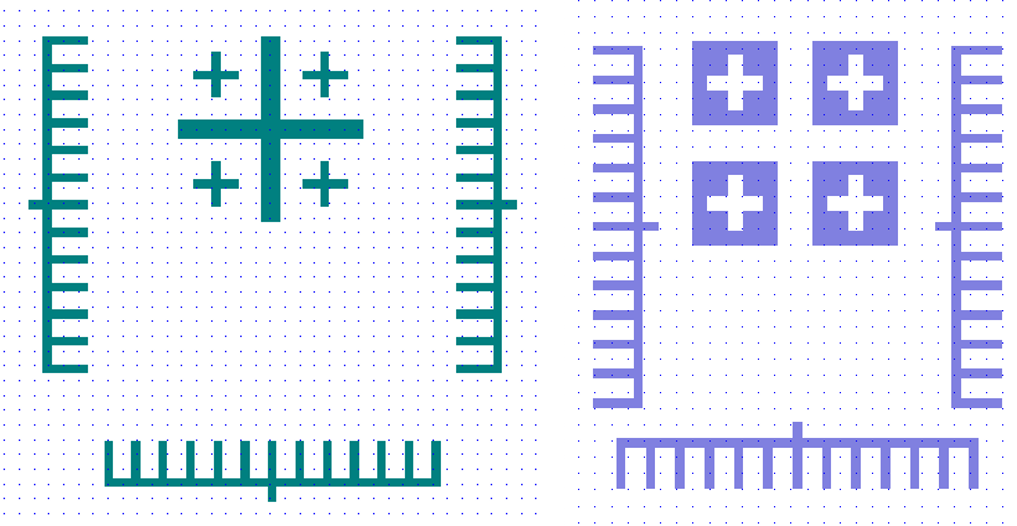
\includegraphics[width=0.3\textwidth]{figures/CleWin_alignment_marks.png}
    \caption{
        Alignment marks for layer 1 on the left and layer 2 on the right. 
        The design allows quantification of the alignment error.
        These marks are the Verniers design. 
    }
    \label{fig:CleWin_alignment_marks}
\end{figure}

\newpage


\subsection{GaAs contact layer etch}
\label{methods:wet_etch}
The heavily p-doped GaAs layer at the top of the metal stack was etched away to allow light to pass out of the LED.
The deposited Au fingers were measured to be 250 nm high in the profilometer.
Measuring the Au height was important for the later measurement of the etch depth of the 100 nm GaAs layer.
The Au fingers were protected with a positive photoresist before the wet etch.
Optimal dose for the positive photoresist was found to be 130 mJ/cm$^2$.
The preperation was done with the following steps:
\begin{enumerate}
    \item Cleaned the sample with IPA.
    \item Dehydration baked at 115 \textdegree C for 5 minutes.
    \item Spin coated SPR 700 resist at 4000 rpm for 34 seconds with 1000 rpm/s acceleration.
    \item Soft baked at 95 \textdegree C for 1 minute.
    \item Aligned the pattern in the MLA. The alignment marks were badly damaged, so the alignment was not perfect. % See \autoref{fig:align_marks}.
    \item Exposed the pattern at 130 mJ/cm$^2$ in the MLA.
    \item Post exposure baked at 115 \textdegree C for 1 minute.
    \item Developed in maD-332S developer for 30 seconds.
    \item Optical inspected the pattern to see if it covered the Au fingers.
\end{enumerate}

Quantification of the misalignment with the Verniers were tried, but the Verniers were too badly damaged to get any number out.
The wet etch was done at the chemical clanroom at NTNU NanoLab, with NH$_3$:H$_2$O$_2$:H$_2$0 in 3:1:300 ratio.
The ammonium hydroxide was 30\%.
The etch depth was tested on the GaAs dummy sample, and measured with the profilometer to figure out an etch time which would remove 100 nm of GaAs.
The GaAs dummy was etched 50 nm at the first run, thus the time was doubled for the LED etch to achieve 100 nm.
The etch steps were as follows:

\begin{enumerate}
    \item 3 mL 30\% NH$_3$ was added to the etch tank with 300 ml H$_2$O.
    \item 1 mL H$_2$O$_2$ was added to the etch tank.
    \item The sample was placed in the etch tank for 90 seconds.
    \item The sample was rinsed with H$_2$O and cleaned on the backside.
    \item The protective photoresist was removed with acetone and IPA before profilometer measurement.
    \item The etch depth was measured with the profilometer.
\end{enumerate}



\subsection{Backside contact formation}
\label{methods:backside_metallization}
The backside of the LED sample was metallized with a Pd/Ge/Ti/Pt/Au stack to form the backside contact.
The positive photoresist SPR 700 was used to protect the frontside, using the following steps:
\begin{enumerate}
    \item Cleaned the sample with acetone and IPA.
    \item Dehydration baked at 115 \textdegree C for 5 minutes.
    \item Spin coated SPR 700 resist at 4000 rpm for 34 seconds with 1000 rpm/s acceleration.
    \item Soft baked at 95 \textdegree C for 1 minute.
    \item No exposure was done, since the whole frontside needed to be protected.
    \item Post exposure baked at 115 \textdegree C for 1 minute.
    \item Developed in maD-332S developer for 30 seconds.
    \item Optically inspected the pattern to see if the whole frontside was covered.
    \item Backside metallization was done by the teaching assistants.
\end{enumerate}


\subsection{Mesa etch, PECVD passivation deposition, and contact annealing}
\label{methods:PECVD}
In one session the the mesa was etched, the passivation layer deposited and the contacts annealed.
The mesa etch was done with a wet etch with H$_3$PO$_4$:H$_2$O$_2$:H$2$O 5:5:15, with the goal of separating the 16 LEDs.
The mesa etch had to get through the two p-doped Al$_{0.7}$Ga$_{0.3}$As layers, i.e. had to be deeper than 3 \textmu m.
The preperation for the mesa etch was to add a positive photoresist mesa mask, which was done in the following steps:

\begin{enumerate}
    \item Cleaned the sample with acetone and IPA.
    \item Dehydration baked at 115 \textdegree C for 5 minutes.
    \item Spin coated SPR 700 resist at 4000 rpm for 34 seconds with 1000 rpm/s acceleration.
    \item Soft baked at 95 \textdegree C for 1 minute.
    \item Aligned the pattern in the MLA.
    \item Exposed the pattern at 130 mJ/cm$^2$ in the MLA.
    \item Post exposure baked at 115 \textdegree C for 1 minute.
    \item Developed in maD-332S developer for 30 seconds.
    \item Optically inspected the pattern to see if it covered the LEDs.
\end{enumerate}

The mesa etch and passivation deposition was done in parallel.
The wet etch was first done on the GaAs dummy to test the etch time, where it was found that 1 minute 30 seconds would be sufficient to etch through the two p-doped layers.
The thickness aim for the passivation layer was 253 nm. 
The following steps were done:

\begin{enumerate}
    \item Deposited Si$_3$N$_4$ passivation layer on Si to find an optimal layer thickness. The recipe used was "(OPT) Si3N4" for 18 minutes and 35 seconds.
    \item Wet etched the dummy to find a suitable etch time. This etch time was 1 minute 15 seconds, which was increased by 15 seconds for the LED etch.
    \item The wet etch was done with H$_3$PO$_4$:H$_2$O$_2$:H$2$O 5:5:15 mL.
    \item The resist was stripped of the dummy, and the etch depth was measured with the profilometer.
    \item The inferometer was used to measure the passivation layer deposition thickness.
    \item The LED was mesa wet etched as the dummy was, but with 1 minutes 30 seconds etch time.
    \item The etch depth was controlled to be deeper than 3 \textmu m in the profilometer.
    \item PECVD passivation layer deposition was done on the LED and the dummy with the same recipe and time as the Si test, because the recipe was found to be good enough.
    \item The last step was the contact annealing, which was done with warm up to 420 \textdegree C, and 30 seconds annealing at 420 \textdegree C, before cooling down to room temperature.
\end{enumerate}



\subsection{Planarization and passivation layer etch}
\label{methods:Planarization}

The passivation layer HF etch was done by the teaching assistants.
The planarization and preperation for the passivation layer etch was to add a thick positive photoresist with a mask opening on the bottom bus bar, and was done in the following steps:

\begin{enumerate}
    \item Cleaned the sample with acetone and IPA.
    \item Dehydration baked at 150 \textdegree C for 5 minutes.
    \item Spin coated AZ5214E positive resist at 1000 rpm for 34 seconds with 250 rpm/s acceleration.
    \item Soft baked at 95 \textdegree C for 1 minute.
    \item Exposed the pattern at 80 mJ/cm$^2$ in the MLA.
    \item Developed in 70:30 ma-D 332S:H$_2$O developer for 1 minute 30 seconds.
    \item Hard baked at 175 \textdegree C for 15 minutes.
    \item Optical inspection of the pattern.
    \item Teaching assistants preformed HF etch to expose the Au in the bottom bus bar.
\end{enumerate}



\subsection{Pad metallization}
\label{methods:pad_metallization}

Lithography on the LED sample was done to prepare for the pad metallization.
The teaching assistants did the pad metallization.
The preparation was to make a negative photoresist mask for the pad metallization, and was done in the following steps:
\begin{enumerate}
    \item Cleaned the sample with IPA.
    \item Dehydration baked at 115 \textdegree C for 5 minutes.
    \item Spin coated MAN 440 resist at 4000 rpm for 30 seconds with 1000 rpm/s acceleration.
    \item Soft baked at 95 \textdegree C for 1 minute.
    \item Exposed the pattern at 1300 mJ/cm$^2$ in the MLA
    \item Developed in maD-332S developer for 5 minutes.
    \item Optical inspected the pattern to see if the pattern covered the bottom bus bar and an area below.
    \item Handed in the sample to the teaching assistants, who did the pad metallization with Ti/Au, with 30 nm Ti and 500 nm Au.
    \item Lift-off was done with acetone.
\end{enumerate}


\subsection{LED testing/characterization}
\label{methods:LED_testing}

The final LED sample was tested using a Keithley 2450 SourceMeter, a probe, and an optical microscope.
Initially, there was no measured contact in the LED between the frontside and the backside.
The voltage was then turned up to 10 V, which warmed up the LED and gave contact. 
Using the SourceMeter, the voltage was swept from -1 V to 3 V, while the measured current was recorded.
The measuring was automatically stopped when a current of 30 mA was reached.
The results were then plotted as an IV-curve.
Two of the LEDs was measured this way. 

The LED was turned on with 1.71 V and 30 mA, and images was taken with an iPhone.